\documentclass{standalone}
\usepackage{tikz}
\usetikzlibrary{patterns, positioning}


\begin{document}
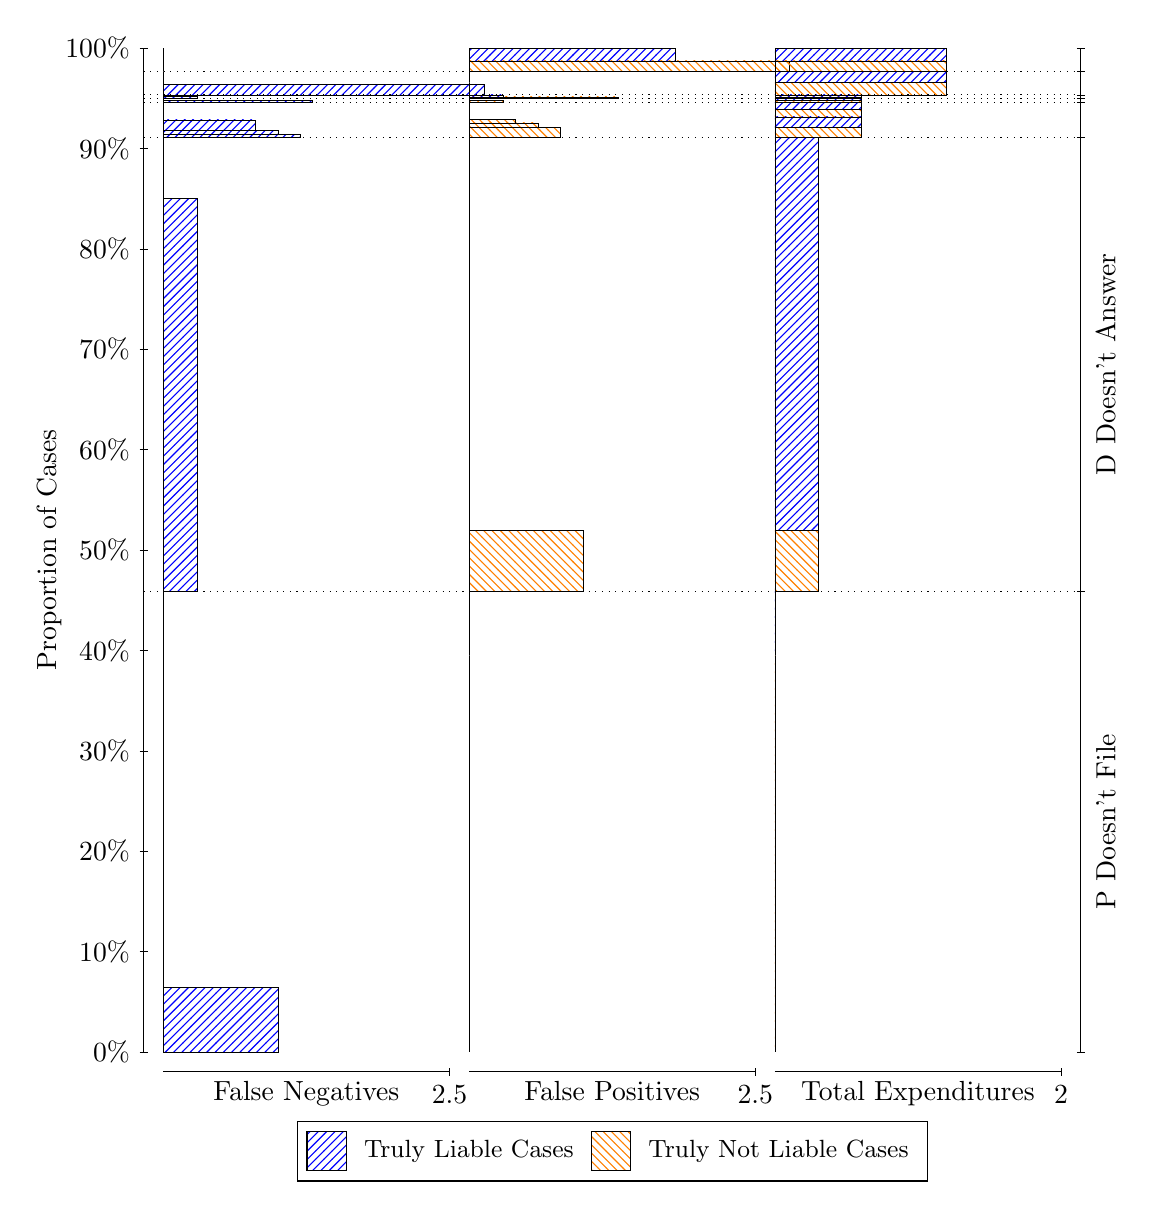
\begin{tikzpicture}
\draw[black, very thin] (1.5,1.75) -- (1.5,14.5);
\node[rotate=90, text=black, anchor=center] at (0.3, 8.125) {Proportion of Cases};
\draw[black, very thin] (1.45,1.75) -- (1.55,1.75);
\node[text=black, anchor=east] at (1.45, 1.75) {0\%};
\draw[black, very thin] (1.45,3.025) -- (1.55,3.025);
\node[text=black, anchor=east] at (1.45, 3.025) {10\%};
\draw[black, very thin] (1.45,4.3) -- (1.55,4.3);
\node[text=black, anchor=east] at (1.45, 4.3) {20\%};
\draw[black, very thin] (1.45,5.575) -- (1.55,5.575);
\node[text=black, anchor=east] at (1.45, 5.575) {30\%};
\draw[black, very thin] (1.45,6.85) -- (1.55,6.85);
\node[text=black, anchor=east] at (1.45, 6.85) {40\%};
\draw[black, very thin] (1.45,8.125) -- (1.55,8.125);
\node[text=black, anchor=east] at (1.45, 8.125) {50\%};
\draw[black, very thin] (1.45,9.4) -- (1.55,9.4);
\node[text=black, anchor=east] at (1.45, 9.4) {60\%};
\draw[black, very thin] (1.45,10.675) -- (1.55,10.675);
\node[text=black, anchor=east] at (1.45, 10.675) {70\%};
\draw[black, very thin] (1.45,11.95) -- (1.55,11.95);
\node[text=black, anchor=east] at (1.45, 11.95) {80\%};
\draw[black, very thin] (1.45,13.225) -- (1.55,13.225);
\node[text=black, anchor=east] at (1.45, 13.225) {90\%};
\draw[black, very thin] (1.45,14.5) -- (1.55,14.5);
\node[text=black, anchor=east] at (1.45, 14.5) {100\%};

\draw[black, very thin] (13.4,1.75) -- (13.4,14.5);
\draw[black, very thin] (13.35,1.75) -- (13.45,1.75);
\node[anchor=west] at (13.35, 1.75) {};
\draw[black, very thin] (13.35,7.6006) -- (13.45,7.6006);
\node[anchor=west] at (13.35, 7.6006) {};
\draw[black, very thin] (13.35,13.367) -- (13.45,13.367);
\node[anchor=west] at (13.35, 13.367) {};
\draw[black, very thin] (13.35,13.811) -- (13.45,13.811);
\node[anchor=west] at (13.35, 13.811) {};
\draw[black, very thin] (13.35,13.859) -- (13.45,13.859);
\node[anchor=west] at (13.35, 13.859) {};
\draw[black, very thin] (13.35,13.905) -- (13.45,13.905);
\node[anchor=west] at (13.35, 13.905) {};
\draw[black, very thin] (13.35,14.2) -- (13.45,14.2);
\node[anchor=west] at (13.35, 14.2) {};
\draw[black, very thin] (13.35,14.5) -- (13.45,14.5);
\node[anchor=west] at (13.35, 14.5) {};

\draw[black, very thin, pattern color=blue, pattern=north east lines] (1.75,1.75) rectangle (3.2033,2.5657);
\draw[black, very thin, pattern color=orange, pattern=north west lines] (1.75,2.5657) rectangle (1.75,7.6006);
\draw[black, very thin, pattern color=blue, pattern=north east lines] (1.75,7.6006) rectangle (2.186,12.593);
\draw[black, very thin, pattern color=orange, pattern=north west lines] (1.75,12.593) rectangle (1.75,13.367);
\draw[black, very thin, pattern color=blue, pattern=north east lines] (1.75,13.367) rectangle (3.494,13.405);
\draw[black, very thin, pattern color=blue, pattern=north east lines] (1.75,13.405) rectangle (3.2033,13.458);
\draw[black, very thin, pattern color=blue, pattern=north east lines] (1.75,13.458) rectangle (2.9127,13.587);
\draw[black, very thin, pattern color=orange, pattern=north west lines] (1.75,13.587) rectangle (1.75,13.811);
\draw[black, very thin, pattern color=blue, pattern=north east lines] (1.75,13.811) rectangle (3.6393,13.833);
\draw[black, very thin, pattern color=orange, pattern=north west lines] (1.75,13.833) rectangle (1.75,13.859);
\draw[black, very thin, pattern color=blue, pattern=north east lines] (1.75,13.859) rectangle (2.186,13.884);
\draw[black, very thin, pattern color=orange, pattern=north west lines] (1.75,13.884) rectangle (1.75,13.905);
\draw[black, very thin, pattern color=blue, pattern=north east lines] (1.75,13.905) rectangle (5.8193,14.042);
\draw[black, very thin, pattern color=orange, pattern=north west lines] (1.75,14.042) rectangle (1.75,14.2);
\draw[black, very thin, pattern color=orange, pattern=north west lines] (1.75,14.2) rectangle (1.75,14.338);
\draw[black, very thin, pattern color=blue, pattern=north east lines] (1.75,14.338) rectangle (1.75,14.5);
\draw[black, very thin, pattern color=orange, pattern=north west lines] (5.6333,1.75) rectangle (5.6333,6.7849);
\draw[black, very thin, pattern color=blue, pattern=north east lines] (5.6333,6.7849) rectangle (5.6333,7.6006);
\draw[black, very thin, pattern color=orange, pattern=north west lines] (5.6333,7.6006) rectangle (7.0867,8.3741);
\draw[black, very thin, pattern color=blue, pattern=north east lines] (5.6333,8.3741) rectangle (5.6333,13.367);
\draw[black, very thin, pattern color=orange, pattern=north west lines] (5.6333,13.367) rectangle (6.796,13.496);
\draw[black, very thin, pattern color=orange, pattern=north west lines] (5.6333,13.496) rectangle (6.5053,13.549);
\draw[black, very thin, pattern color=orange, pattern=north west lines] (5.6333,13.549) rectangle (6.2147,13.59);
\draw[black, very thin, pattern color=blue, pattern=north east lines] (5.6333,13.59) rectangle (5.6333,13.811);
\draw[black, very thin, pattern color=orange, pattern=north west lines] (5.6333,13.811) rectangle (6.0693,13.837);
\draw[black, very thin, pattern color=blue, pattern=north east lines] (5.6333,13.837) rectangle (5.6333,13.859);
\draw[black, very thin, pattern color=orange, pattern=north west lines] (5.6333,13.859) rectangle (7.5227,13.88);
\draw[black, very thin, pattern color=blue, pattern=north east lines] (5.6333,13.88) rectangle (6.0693,13.905);
\draw[black, very thin, pattern color=orange, pattern=north west lines] (5.6333,13.905) rectangle (5.6333,14.062);
\draw[black, very thin, pattern color=blue, pattern=north east lines] (5.6333,14.062) rectangle (5.6333,14.2);
\draw[black, very thin, pattern color=orange, pattern=north west lines] (5.6333,14.2) rectangle (9.7027,14.338);
\draw[black, very thin, pattern color=blue, pattern=north east lines] (5.6333,14.338) rectangle (8.2493,14.5);
\draw[black, very thin, pattern color=orange, pattern=north west lines] (9.5167,1.75) rectangle (9.5167,6.7849);
\draw[black, very thin, pattern color=blue, pattern=north east lines] (9.5167,6.7849) rectangle (9.5167,7.6006);
\draw[black, very thin, pattern color=orange, pattern=north west lines] (9.5167,7.6006) rectangle (10.062,8.3741);
\draw[black, very thin, pattern color=blue, pattern=north east lines] (9.5167,8.3741) rectangle (10.062,13.367);
\draw[black, very thin, pattern color=orange, pattern=north west lines] (9.5167,13.367) rectangle (10.607,13.496);
\draw[black, very thin, pattern color=blue, pattern=north east lines] (9.5167,13.496) rectangle (10.607,13.626);
\draw[black, very thin, pattern color=orange, pattern=north west lines] (9.5167,13.626) rectangle (10.607,13.72);
\draw[black, very thin, pattern color=blue, pattern=north east lines] (9.5167,13.72) rectangle (10.607,13.811);
\draw[black, very thin, pattern color=orange, pattern=north west lines] (9.5167,13.811) rectangle (10.607,13.837);
\draw[black, very thin, pattern color=blue, pattern=north east lines] (9.5167,13.837) rectangle (10.607,13.859);
\draw[black, very thin, pattern color=orange, pattern=north west lines] (9.5167,13.859) rectangle (10.607,13.88);
\draw[black, very thin, pattern color=blue, pattern=north east lines] (9.5167,13.88) rectangle (10.607,13.905);
\draw[black, very thin, pattern color=orange, pattern=north west lines] (9.5167,13.905) rectangle (11.697,14.062);
\draw[black, very thin, pattern color=blue, pattern=north east lines] (9.5167,14.062) rectangle (11.697,14.2);
\draw[black, very thin, pattern color=orange, pattern=north west lines] (9.5167,14.2) rectangle (11.697,14.338);
\draw[black, very thin, pattern color=blue, pattern=north east lines] (9.5167,14.338) rectangle (11.697,14.5);
\draw[black, dotted] (1.5,7.6006) -- (13.4,7.6006);
\draw[black, dotted] (1.5,13.367) -- (13.4,13.367);
\draw[black, dotted] (1.5,13.811) -- (13.4,13.811);
\draw[black, dotted] (1.5,13.859) -- (13.4,13.859);
\draw[black, dotted] (1.5,13.905) -- (13.4,13.905);
\draw[black, dotted] (1.5,14.2) -- (13.4,14.2);
\draw[black, very thin] (1.75,1.5) -- (5.3833,1.5);
\node[text=black, anchor=north] at (3.5667, 1.5) {False Negatives};
\draw[black, very thin] (5.3833,1.45) -- (5.3833,1.55);
\node[text=black, anchor=north] at (5.3833, 1.45) {2.5};

\draw[black, very thin] (5.6333,1.5) -- (9.2667,1.5);
\node[text=black, anchor=north] at (7.45, 1.5) {False Positives};
\draw[black, very thin] (9.2667,1.45) -- (9.2667,1.55);
\node[text=black, anchor=north] at (9.2667, 1.45) {2.5};

\draw[black, very thin] (9.5167,1.5) -- (13.15,1.5);
\node[text=black, anchor=north] at (11.333, 1.5) {Total Expenditures};
\draw[black, very thin] (13.15,1.45) -- (13.15,1.55);
\node[text=black, anchor=north] at (13.15, 1.45) {2};

\node[text=black, centered, rotate=90] at (13.72, 4.6753) {P Doesn't File};
\node[text=black, centered, rotate=90] at (13.72, 10.484) {D Doesn't Answer};






\draw (7.449999999999999,1.5) node[draw=none] (baseCoordinate) {};
\begin{scope}[align=center]
        \matrix[scale=0.5, draw=black, below=0.5cm of baseCoordinate, nodes={draw}, column sep=0.1cm]{
            \node[rectangle, draw, minimum width=0.5cm, minimum height=0.5cm, pattern color=blue, pattern=north east lines] {}; &
            \node[draw=none, font=\small, text=black] (B) {Truly Liable Cases}; &
            \node[rectangle, draw, minimum width=0.5cm, minimum height=0.5cm, pattern color=orange, pattern=north west lines] {}; &
            \node[draw=none, font=\small, text=black] (B) {Truly Not Liable Cases}; \\
            };
\end{scope}

\end{tikzpicture}
\end{document}